
\chapter{Metodologia de Trabalho}
%Para a organização do trabalho foi utilizada a técnica de desenvolvimento ágil SCRUM
De forma a organizar todo o trabalho a desenvolver visto que este é dividido com mais uma colega, 
foi então utilizada a técnica de desenvolvimento ágil, conseguindo assim organizar todas as tarefas 
entre os elementos de desenvolvimento do projeto.

\section{Ferramentas de trabalho utilizadas}

A organização de todas as tarefas, foi realizada na ferramente Github Projetcs, esta 
permite ligar um projeto a um repositório de Github, conseguindo também personalizar completamente todo 
o projeto e parâmetros das tarefas o que permite uma organização minuciosa destas.

O Microsoft Excel foi também utilizado para a engenharia de software onde foram descritos os requisitos 
do projeto, user stories e também a especificação de casos de uso. Esta ferramenta foi também utilizada 
para a organização de reuniões com o cliente e redação de tópicos a abordar e abordados nesta.

Para o desenvolvimento do design do software foi utilizado a ferramenta figma, que permite o design de 
todas as componentes tendo em conta as reais dimensões de um dispositivo. Esta ferramenta 
permite também criar uma apresentação interativa que consegue demonstrar o comportamento da aplicação 
como completamente desenvolvida, dando também suporte à implementação.

O draw.io foi também utilizado para o desenho das arquiteturas do projeto tendo se revelado de grande auxílio 
visto que este permite uma grande liberdade no desenho. Esta ferramenta permite também 
conexão com github conseguindo assim facilmente guardar estes projetos e ter acesso a partir de qualquer 
dispositivo.

A engenharia de software foi realizada utilizando Visual Studio paradigm, esta é uma ferramenta muito 
completa contendo modelos e regras para a engenharia de software. Esta ferramenta tornou-se um grande 
auxílio no desenvolvimento da base de dados, pois é possível desenhar o modelo e exportar para um ficheiro 
de criação de base de dados.

\newpage

\section{Planificação do trabalho}

De forma a obter uma visão geral do projeto e uma previsão de finalização foi realizada uma planificação 
expectável de tarefas. Visto que o supervisor de estágio propôs uma divisão do projeto por etapas, as 
tarefas de cada etapa eram definidas no início da etapa. O objetivo seria melhorar a solução ao fim de 
cada etapa implementando novas funções, pelo que a cada nova etapa todo o processo de engenharia de 
software teria de se repetir.

Sendo assim as etapas são:
\begin{itemize}
    \item Etapa 1 - Desenvolvimento de fórum e catálogo de produtos - Figura~\ref{fig:1}.
    
\end{itemize}

\begin{figure}[htb]
    \centering
    
    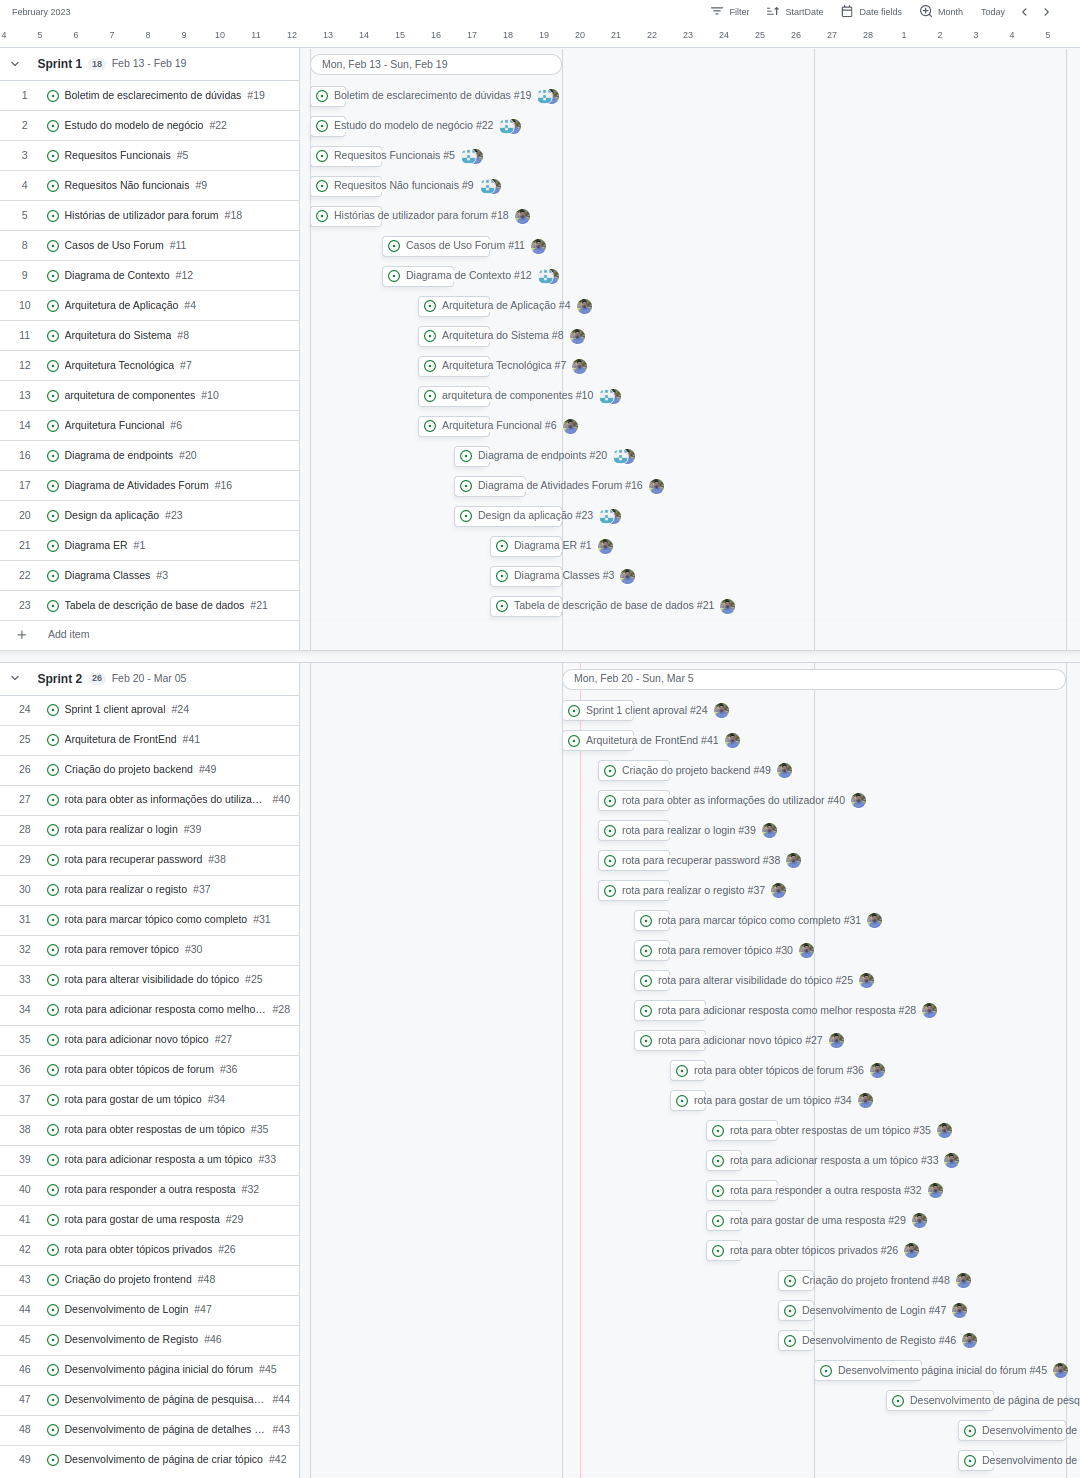
\includegraphics[width=0.75\textwidth]{images/etapa1_sprint_planning.png}
    \caption{Planeamento de sprint da etapa 1}
    \label{fig:1}
\end{figure}



